\graphicspath{{chapters/02_introduction/images}}
\chapter{Introduction}

% The Introduction provides the background to the research work (at least 5 pages, not more than 10). 

% TODO: Check if needed anymore
% \section{Epigenetic factors and chromatin organization}
% Albeit DNA sequence is what actually defines the sequence of the transcript obtained from each gene, it is well know that it is not the only factor regulating gene expression and, consequently, organism phenotype. There exist, in fact, multiple epigenetic factors, meaning factors that act upon gene expression regulation without being encoded directly by the DNA sequence. Some of these factors are heritable, while other are acquired throughout life. Epigenetic factors can be tissue specific and in fact they are a major player in cell differentiation. Among these factors there are DNA methylation, histone modifications and chromatin organization\cite{epigeneticbook2020}.

% \subsection{DNA methylation}
% Although not the only one, DNA methylation is by far the most studied DNA modification. DNA methylation refers to the addition of methyl groups to the C-5 position of cytosine residues, especially those followed by a guanine residue (CpG sites). Cytosine methylation affects protein binding affinity, either increasing or decreasing it. It is regulated by a complex enzymatic machinery composed of writers (enzymes which add methyl groups), erasers (enzymes which remove methyl groups) and readers (proteins whose binding affinity to a region depends on its methylation state). Physiologically, DNA methylation is responsible for mechanisms such as silencing of retroviral elements, regulation of tissue-specific gene expression, genomic imprinting and X chromosome inactivation\cite{methylationgeneral2012, methylationhistoric2022}. When dysregulated, DNA methylation can cause or contribute to many pathological conditions, such as genesis and/or progression of cancer\cite{methylationcancer2016, methylationcancer2021} or other diseases such as stress and depression\cite{methylationdepression2023}, retinal diseases\cite{methylationretinal2023}, congenital hearth disease \cite{methylationheart2021} and many others\cite{epigeneticbook2020}.

% \subsection{Histone modifications}
% The DNA in the nucleus is not in a completely unwound state, but rather in a variably-condensed one called chromatin. Stretches of 145-147 bp of DNA are wrapped around proteic octamers composed of proteins called histones; these structures, called nucleosome, are the first level of chromatin condensation\cite{chromatinstructure2018}. Each histone is composed of a core portion, around which the DNA is wrapped, and a tail portion, which is 20-40 aminoacids long, exposed to the nucleosol. The aminoacidic composition of the tails is what confers them an electronic charge, impacting DNA binding and thus chromatin condensation level. It is in fact possible to define, on a mesoscale level, two types of chromatin, heterocromatin and eucromatin; the former is a more condensed state, and for this reason genes located within this region are less transcribed since transcription factors binding is impeded, while the latter is the less condensed state, favouring gene accessibility and transcription. The chromatin state of a genomic region can change overtime and one major factor in defining these shifts are covalent modifications of histone tails, notably acetylation, phosphorylation, methylation, SUMOylation and ubiquitination\cite{histonemodifications2020}. 

With the passing of time, it has become more and more evident that the way DNA is organized in the nucleous is not inconsequential, but rather a fundamental aspect especially, but not exclusively, for gene transcription\cite{chromatinfiber2015}. The way DNA is compacted into chromatin and folded, for instance, can affect whether genes are accessible to the RNA-polymerase, or whether regulatory sequences are accessible to transcription factors; moreover, chromatin conformation defines which regulatory elements are close enough to their target to exert their action.

Firstly, how DNA is shaped into chromatin and how this is organized into the nucleous will be discussed. Then, a subset of experimental techniques used to study chromatin conformation, the so-called ligation-based methods, and one in particular, Hi-C, will be described. The next topic will be the way data coming from these techniques is usually stored and analyzed. Finally, some background on graph theory and network analysis will be provided, since network sparsification, a network analysis algorithm, is the main point of the data preprocessing pipeline in this work.

\section{Chromatin composition and organization}

\subsection{Nucleosomes and 30-nm chromatin fiber}

it is not the only factor regulating gene expression and, consequently, cell phenotype. There exist, in fact, multiple epigenetic factors, meaning factors that act upon gene expression regulation without being encoded directly by the DNA sequence. Some of these factors are heritable, while other are acquired throughout life. Epigenetic factors can be tissue specific and in fact they are a major player in cell differentiation. Among these factors there are DNA methylation, histone modifications and chromatin organization\cite{epigeneticbook2020}.

The DNA nucleotidic sequence encodes both genes and gene regulatory elements such as enhancers and silencers. The presence itself of these elements though is not enough, since gene and regulatory element need to be in proximity of each other to act, either directly or through protein mediated contact. For this reason chromatin organization itself becomes an epigenetic factor, defining which genomic areas are accessible and which ones are close enough to interact with others. During interphase, chromatin organization is rather complex and characterized by different features depending on the scale it is analysed at\cite{chromatinorganization2019, chromatindevelopment2019}.


\subsection{3D chromatin organization}
The DNA sequence encodes both genes and gene regulatory elements such as enhancers and silencers. The presence itself of these elements though is not enough, since gene and regulatory element need to be in proximity of each other to act, either directly or through protein mediated contact. For this reason chromatin organization itself becomes an epigenetic factor, defining which genomic areas are accessible and which ones are close enough to interact with others. During interphase, chromatin organization is rather complex and characterized by different features depending on the scale it is analysed at\cite{chromatinorganization2019, chromatindevelopment2019}.

At a very broad scale, chromatin is organized in chromosome territories and compartments. Interphasic chromosomes tend to occupy distinct regions of the nucleus, the so called chromosome territories. Within a chromosome territory, it is possible to distinguish transcriptionally active and inactive regions; regions of the same type tend to interact with each other forming compartments. Compartment A is mostly composed of transcriptionally active regions, with high gene density and active histone modifications. On the other hand compartment B is mostly composed of trascriptionally inactive regions, with lower gene density or gene deserts. Compartments and chromatin states are not necessarily overlapping, even though compartment A tends to be mostly composed of euchromatin and vice versa. Compartment A is frequently found in the interior nuclear space, organized around nuclear speckles, while compartment B is generally found at the periphery of the nucleus, in contact with the nuclear lamina, or close to the nucleolus.

On a smaller scale one can identify two main structures, those being topologically associating domains (TADs) and loop domanis. A TAD is a region of the genome which forms contacts with itself more frequently that with other regions. [WHAT ARE THEY AND WHY ARE THEY IMPORTANT] A loop is a cohesin-mediated interaction between paired CCCTC-binding factor (CTCF) proteins. [AGAIN, EXACTLY WHAT ARE THEY AND WHY ARE THEY IMPORTANT]

Finally at the lowest scale one can define promoter enhancer contacts [WHICH ARE EXACTLY WHAT YOU THINK THEY ARE.]

WHY STUDYING CHROMOSOME CONFORMATION.

\begin{figure}
  \centering
  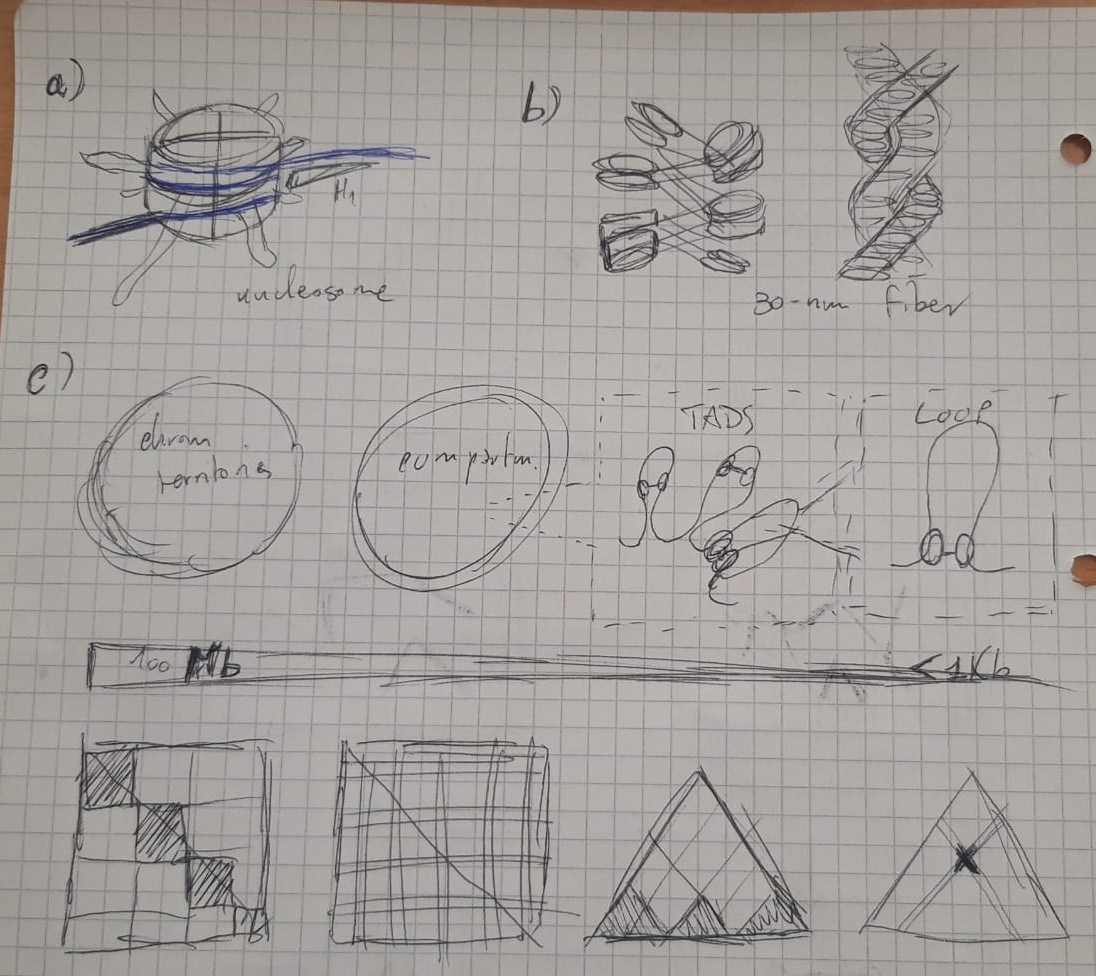
\includegraphics[width=1\textwidth]{chromatin_organization.jpeg}
  \caption{\textbf{Chromatin organization leveles}. Different levels of chromatin structure organization at different scales. (a) The nucleosome is the lower level of chromatin organization; a nucleosome is constituted by DNA wrapped around a proteic octamer plus a linker regions and a H1 histone. (b) The 30-nm chromatin fiber is composed of several nucleosomes and can have varying levels of compactness. (c) Different 3D-organization levels can be found at different scales. Organization levels in decreasing order of magnitude and how they can be visualized on a contact matrix; from left to right, chromosomal territories, A/B compartments, Topologically Associating Domains (TADs), loops. Some lorem ipsum test just to visualize the caption size the way it will probably be once it is complete. Some lorem ipsum test just to visualize the caption size the way it will probably be once it is complete. Some lorem ipsum test just to visualize the caption size the way it will probably be once it is complete. Some lorem ipsum test just to visualize the caption size the way it will probably be once it is complete. Some lorem ipsum test just to visualize the caption size the way it will probably be once it is complete.}
\end{figure}

\section{Ligation-based methods for the study of chromatin organization}

There exist plenty of methods to study chromatin organization, which can be divided into imaging-based, ligation-based and ligation-free methods. Ligation-based methods stem from one original method, that is chromosome conformation capture, which has been overtime modified to increase resolution and throughput. From the derived methods, Hi-C was the first which allowed to study interactions on a genome-wide scale.

\subsection{Chromosome conformation capture}
Chromosome conformation capture (3C), the original ligation-based method, is a technique which allows to study interactions among genomic regions through chromatin crosslinking and proximity ligation\cite{3coriginal2002}. The main steps of the original protocol are the following:
\begin{itemize}\tightlist
  \item formaldehyde fixation of isolated, intact nuclei. Formaldehyde causes a crosslinking reaction which stabilizes protein-protein and protein-DNA interactions; this means that DNA regions will be in proximity to each other thanks to their protein mediated interactions. 
  \item chromatin digestion through a restriction enzyme (EcoRI).
  \item fragment ligation at very low DNA concentration. In this condition, ligation among DNA fragments crosslinked through proteins is heavily favoured, given that they will always be in proximity of each other.
  \item crosslinking reversion and DNA purification.
  \item quantitative PCR using locus specific primers. The contact frequency among two loci is given by the ratio with the quantity obtained through quantitative PCR on a control.
\end{itemize}
It is important to notice that this is a 1 vs 1 technique, meaning that only one pair of loci can be analysed at a time; moreover each comparison requires 2 quantitative PCRs (sample and control) and a pair of locus specific primers, thus requiring some prior knowledge of the target. For these reason the technique is very limited and was overtime modified to become 1 vs all (4C\cite{4cprotocol2006}), many vs many (5C\cite{5cprotocol2006}) and then finally all vs all with Hi-C.


\subsection{Hi-C protocol}
Hi-C was the first ligation-based method to allow a genome wide study of chromatin interactions. It differs from the original 3C technique mostly for nucleus lysis using sodium dodecyl sulfate (SDS), the usage of biotin to tag and enrich ligation products and for the usage of sequencing for quantification rather than quantitative PCR\cite{hicoriginal2009}. An optimization of the original Hi-C protocol is in situ Hi-C, whose main difference is that it does not perform nuclear lysis; this reduces the number of ligation events due to random interaction of DNA fragments in solution, while at the same time reducing the reaction volumes and increasing the number of captured interactions\cite{insituhic2014}. The in-situ Hi-C protocol can be summarised as follows:

\begin{itemize}\tightlist
  \item DNA crosslinking on intact nuclei
  \item chromatin digestion through a restriction enzyme
  \item fill sticky ends at the restriction sites with biotinilated nucleotides
  \item proximity ligation
  \item crosslinking reversion, DNA shearing (to 400 bp size) and fragment pulldown using streptavidin beads
  \item pair-end sequencing to obtain chimeric reads
\end{itemize}
 
Altough in-situ Hi-C is the most common variant of the Hi-C protocol, it is not the only one. Of particular notice is Micro-C\cite{microc2015}, which uses micrococcal nuclease as a restriction enzyme for DNA digestion. This means that all linker DNA is degraded and only interactions among nucleosomes are kept. Given the smaller fragment size, this results in a higher resolution at shorter genomic distances, while long range interactions are poorly captured, making this technique complementary to Hi-C rather than a replacement.

% TODO: Add image about the two protocols

\section{Hi-C data storage and analysis}

Handling Hi-C sequencing data is rather challenging for several reasons, both in terms of storage and analysis itself. This type of data requires different processing steps and file formats with respect to standard genomic DNA sequencing, requiring therefore specifically designed tools and algorithms. The following subsections cover the typical steps to obtain contact matrices strarting from sequencing raw data and some of the commonly performed analyses\cite{hicprocessing2018}. The most common representations and file formats for Hi-C data are also presented.

\subsection{Sequence alignment and binning}
The sequencing step of a Hi-C procedure generally yields some billions of paired-end reads. The fragments from which the reads are derived are chimeric, meaning that they are composed of sequences from regions which are (typically) not genomically contiguous. For this reason it is assumed that the two paired-ends can be mapped independently using standard tools such as bowtie. Still, it is important to notice that, especially for longer reads, the junction among the two interacting genomic regions might fall within one of the paired reads, making it chimeric. Chimeric reads are difficult to map and require apposite strategies which are implemented by Hi-C data specific tools in order to avoid losing a huge amount of information. The aligned reads are then filtered using both standard DNA sequencing criteria, such as base quality and PCR artifacts, as well as Hi-C specific ones, such as self-ligation products, compatibility with undigested chromatin\cite{readfiltering2013} or more elaborate ones\cite{complexfiltering2017}.

Binning is the next main step performed; the genome is divided into regions, the bins, and each read is substituted with the bin it falls into. The objective of this procedure is to discretize the signal in order to reduce noise, since it is easier to define the contact frequencies among two regions if they have well defined boundaries (even though this comes with a reduction in resolution).
Although using bins of variable size is an option, fixed-size bins are the more common choice since they are easier to work with. The chosen bin size will affect the resolution of the final contact matrix. The bigger the bin size, the lower the resolution but the more robust the signal; conversely, the smaller the bin size, the higher the resolution but the noisier the signal. Virtually any bin size coul be used, though common sizes span the order of some kilobases (1-10 kb). Bins are assigned a progressive numeric id, from 0 to the number of bins minus 1, to avoid having to refer to them with the entire genomic coordinates they correspond to; sticking to 10 kb resolution, chromosome 1 from base 1 to 10000 would be bin 0, chromosome 1 from base 10001 to 20000 would be bin 1 and so on. After binning, the aligned paired-end reads are thus substituted by pairs of bin ids, and since there is a finite number of bins, it is possible to count the number of occurrencies of each pair of ids; this basically corresponds to counting how many times the two genomic regions represented by the bins have been found in contact with each other, thus this number is the absolute frequency of their interaction. 

\subsection{Contact matrix and ijv table}

The aligned, filtered and binned Hi-C data che be represented either using a contact matrix or using an \emph{ijv} table; these formats are illustrated and compared in image [ADD IMAGE].

A contact matrix is a symmetric and sparse matrix, with all the bins the genome has been divided into as both rows and columns. This means that each cell of the matrix represents how many times the bin corresponding to its row has been found in contact with the bin corresponding to its column. A contact matrix is usually displayed using a heatmap, where each cell is represented by a colored square with intensity proportional to the cell value. For this reason each cell of the matrix is also refferred to as pixel. Aside from being convenient for visualization purposes, a contact matrix is also convenient to perform row or column-wise operations. For instance, given a certain bin, one can easily obtain the list of interacting bins by looking at the non-zero cells in the corresponding row, or one can compute the number of interactions for that bin by summing the values of all cells in the corresponding row. On the other hand, a contact matrix is not a convenient way to store data. The size of the contact matrix scales quadratically with the number of bins the genome has been divided into; with an itermediate bin size of 10 kb, a contact matrix corresponding to the entire human genome has around $10^{11}$ cells. For this reason a contact matrix can become hard to handle and store into memory, especially as the resolution increases.

The \emph{ijv} table is a format which allows for efficient Hi-C data storage by taking advantage of the properties of the contact matrix. Since the contact matrix is symmetric (the bin contacts are not directional), only the upper triagular part of it (the cells on the main diagonal and those above it) can be stored without losing information. Moreover, since it is a sparse matrix, meaning that most cells have value equal to zero, only the cells with non-zero value can be stored. From these consideration one can define an \emph{ijv} table, also called coordinated list format (COO), as a tabular format where each row contains the two bin ids corresponding to the coordinates of the cell and the value associated to it, and only cells with a value greater than zero are stored. This representation drastically reduces the amount of pixels that need to be stored, and can be converted at any point to the full contact matrix version for visualization. Notice that this format is not well suited for row or column-wise operations, since not all the pixels involving a bin are likely to be contiguous. The pixels are in fact ordered in the same way one would encounter them by going over the upper triangular part of the contact matrix from left to right, from top to bottom; this means that the row bin id will always be smaller than or equal to the column bin id, and that the rows are sorted by row bin id, then by column bin id.

\subsection{HDF5 and cooler file formats}
An \emph{ijv} table is a very long one dimensional array, that could theoretically be $n^2$ rows long, where $n$ is the number of bins the genome has been divided into. Although the full possible size is never reached, a plain text representation of an \emph{ijv} table would be rather limiting in terms of I/O speed; for instance, looking for all the interactions of a certain bin might require a full pass of the rows. A better choice is to use of a compressed, indexed binary file format. 

The Hierarchical Data Format version 5 (HDF5) is a binary file format mantained by the HDF group\cite{hdfgroup}. A HDF5 file is organized hierachically just like a file system, with nested groups corresponding to folders and datasets corresponding to tables. A dataset is a table with one or more columns, but whose cells all share the same datatype; in order to represent tables with heterogeneous column datatypes, a typical solution is to create the columns as individual datasets, then fetch rows from them simultaneously. Each dataset can be compressed using different algorithms, the default one being gzip. Both groups and tables can be associated with some metadata, divided into attributes; for this reason the format is dubbed as self-descriptive. For all these reasons, the HDF5 file format is ideal for the storage and quick retrieval of big, heterogeneous datasets, which led to its usage in several fields, sometimes with specialized versions for different applications[CITATIONS].

One such specialized version is the cooler file format, which was introduced in order to facilitate the storage and retrieval of Hi-C data (or any other type of genomically labeled array)\cite{cooler2020}. A cooler file is therefore a HDF5 with a specific structure; each file contains 4 main groups:
\begin{itemize}\tightlist
  \item bins, containing ids and genomic coordinates of the bins the genome was divided into.
  \item pixels, containing the actual contact matrix in \emph{ijv} form.
  \item chroms, containing the chromosomes of the reference genome and their length.
  \item indexes, containing indexes for the pixels group, for faster pixel retrieval.
\end{itemize}
Each of these groups contains several datasets which represent individual columns of a single table, which is a common practice for HDF5 files as previously mentioned; since the group itself merely acts as a container to group the columns, from here on, the term table will be used to refer to the table obtained by joining the individual datasets present in the group.

Each row in the bins table represents one of the bins the genome has been divided into. For each bin, \texttt{chrom}, \texttt{start} and \texttt{end} positions are always specified (e.i. "\texttt{chr1  10001  20000}"), while any number of columns containing additional bin annotations can be present. In general, the package \emph{cooler}, used to create these files, adds some columns with bin weights for normalization purposes (see next subsection), but any other type of annotation, such as the presence of functional elements (e.i. promoters), can be present. While there is not column reserved for bin ids, the index of the bin in the bin table itself is the bin id; this way it becomes easy to retrieve a certain bin by simply knowing its id.

The pixel table is the \emph{ijv} representation of the contact matrix. Each row has exactly three values, those being \texttt{bin1\_id}, \texttt{bin2\_id} and \texttt{count}, where the first two are the ids of the two interacting bins (row and column bin, respectively), while the third is the raw number of contacts found after binning the aligned paired-reads. By referring to the bins via their ids, the pixel table can be drastically simplified, since each bin can be identified using just one column rather than the three necessary to specify the genomic coordinates. At any point, a subset of the pixel table can be converted to the extended form, in which bins are identified by their genomic coordinates, via the process called pixel annotation.

A \texttt{.cool} file contains only one pixels table at one resolution (one bin size). A multiresolution cooler, or \texttt{.mcool} file, is a collection of \texttt{.cool} files referring to the same experiment but at different resolutions. It is itself a single HDF5 file, with a root group called \texttt{resolutions} in which the individual coolers can be found in groups named after the binning resolution. It is important to notice that this format is mostly designed for grouping purposes; the different resolutions are completely independent from each other during processing, therefore working on one does not impact the others. Another specialized form of cooler format is the \texttt{.scool} format, which is instead a collection of \texttt{.cool} (or \texttt{.mcool}) files corresponding to different cells and it is thus used for single cell experiments. 

% TODO: Cite 4D nucleome adopted this format as main one

\subsection{Sequencing biases normalization strategies}

Different bins have different genomic sequences and properties, leading to different sequencing biases. Several normalizations strategies for systematic biases in Hi-C data exist and none of them seems to be a clear cut winner with respect to the others\cite{normalization2020}. These normalization methods can be divided into explicit and implicit methods. 

Explicit methods are methods which correct for a clearly defined set of systematic biases, such as GC content and mappability. The biases are assumed to be independent from each other; thus, for each bias, a normalization factor is computed for each bin, then the normalization factors are combined to obtain the overall bin normalization factor. It is important to notice though, that this type of technique generally considers the bins homogeneous, which even at a fairly low bin sizes might be seen as a major approximation. For instance, it is obvious that a 5 kb genomic sequence could be divided into areas with very distinct GC content; yet a single GC content normalization factor is applied to all reads falling into the bin, disregarding the fact that a read will never cover the entirety of the bin and it might fall in areas with significantly higher of lower GC content than the average for the bin.

Implicit methods are menthods which do not clearly state the systematic biases to correct for. Their assumption is that all systematic biases are recapitulated by sequencing depth, and therefore, making sequencing depth comparable among bins, should correct for all of them, whether they are known or not. This in turn equates to assuming that all genomic regions form the same number of interactions and that there is the same number of copies of each region in the genome (no aneuploidies). This is usually achieved through matrix-balancing methods, a class of mathematical algorithms which try to shape a matrix into some constrained form (in this case, comparable bin coverages) while retaining most of the properties of the original matrix. Among matrix-balancing methods, the most common are iterative correction and eigenvector decomposition (ICE)\cite{ice2012} and Knight-Ruiz (KR)\cite{knightruiz2012}, which are also commonly used as weight columns in \texttt{.cool} files. Matrix-balancing methods are individual-sample normalization approaches and they are generally outperformed by cross-sample normalization ones, especially in regards of reproducibility. Still, individual-sample normalization approaches have the major advantage of usually being significantly faster, also considering the fact that one file has to be normalized only once regardless of how many analyses and comparisons will be performed on it. For this reason matrix-balancing methods are the more common ones.

After computing bin normalization factors, be it through explicit or implicit methods, the pixel counts can be normalized by applying (usually by multiplying) the normalization factors of the two bins consituting the pixel. This entails a further assumption, that is that systematic biases as independent across bins.

\subsection{Hi-C data analysis}

As stated while discussing chromatin organization, different structures and levels of organization are distinguishable depending on the scale the analysis is being conducted at. For this reason, there exist many tools which study one or many of these different aspects of chromatin conformation, though in general the tools can be classified according to whether they can be used to study compartments, TADs, loops or for visualization\cite{hicprocessing2018}.

Compartments are 
[TAD AND LOOP CALLING, MAYBE OTHER]

% TODO: Definitely image of contact matrices (maybe highlighting TAD and LOOP)
% TODO: Definitely image of file structure of cool file

\section{Network analysis}

[INTRO, also semantic of network-graph]
% What is network analysis, graph definition, advantages etc

\subsection{Graph theory concepts}
% TODO: Add node strenght definition
[NODE STRENGTH, NEIGHBOURHOOD, ETC.]

\subsection{Advantages of network analysis}
[LIST THEM AND CURRENT USES IN OTHER FIELDS]

% TODO: Some image for network analysis